%-----------------------------------LICENSE------------------------------------%
%   This file is part of Mathematics-and-Physics.                              %
%                                                                              %
%   Mathematics-and-Physics is free software: you can redistribute it and/or   %
%   modify it it under the terms of the GNU General Public License as          %
%   published by the Free Software Foundation, either version 3 of the         %
%   License, or (at your option) any later version.                            %
%                                                                              %
%   Mathematics-and-Physics is distributed in the hope that it will be useful, %
%   but WITHOUT ANY WARRANTY; without even the implied warranty of             %
%   MERCHANTABILITY or FITNESS FOR A PARTICULAR PURPOSE.  See the              %
%   GNU General Public License for more details.                               %
%                                                                              %
%   You should have received a copy of the GNU General Public License along    %
%   with Mathematics-and-Physics.  If not, see <https://www.gnu.org/licenses/>.%
%------------------------------------------------------------------------------%

%   Use the standalone class for displaying the tikz image on a small PDF.
\documentclass[crop, tikz]{standalone}

%   Import the tikz and pgfplots packages to use for the drawing.
\usepackage{tikz, pgfplots}

% tikz libraries used in the drawing.
\usetikzlibrary{
    angles,              % Drawing angles within triangles.
    quotes,              % Adding labels to angles.
    decorations.markings % Adding fancy braces to lines.
}

%   Begin the document.
\begin{document}

    %   Draw the figure.
    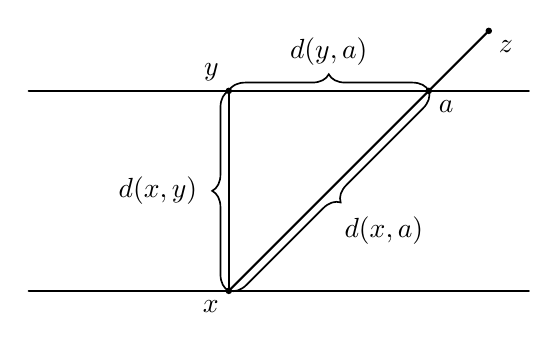
\begin{tikzpicture}[%
        line width=0.6pt,
        line cap=round
    ]
        \coordinate (x) at (0, 0);
        \coordinate (y) at (0, 1in);
        \coordinate (a) at (1in, 1in);
        \coordinate (z) at (1.3in, 1.3in);
        \draw[thick] (-1in, 0) to (1.5in, 0);
        \draw[thick] (-1in, 1in) to (1.5in, 1in);
        \draw[thick] (x) to (y);
        \draw[thick] (x) to (z);
        \draw[decorate, decoration={brace,amplitude=6pt}]
            (x) to node [xshift=-0.9cm] {$d(x,y)$} (y);
        \draw[decorate, decoration={brace,amplitude=6pt}]
            (a) to node [xshift=0.7cm,yshift=-0.5cm] {$d(x,a)$} (x);
        \draw[decorate, decoration={brace,amplitude=6pt}]
            (y) to node [yshift=0.5cm] {$d(y,a)$} (a);
        \draw[fill=black] (x) circle (0.3mm);
        \draw[fill=black] (y) circle (0.3mm);
        \draw[fill=black] (z) circle (0.3mm);
        \draw[fill=black] (a) circle (0.3mm);
        \node at (x) [below left] {$x$};
        \node at (y) [above left] {$y$};
        \node at (a) [below right] {$a$};
        \node at (z) [below right] {$z$};
    \end{tikzpicture}
\end{document}
